\hypertarget{ux8f93ux5165ux548cux8f93ux51fa}{%
\subsection{输入和输出}\label{ux8f93ux5165ux548cux8f93ux51fa}}

\hypertarget{ux8f93ux51fa}{%
\subsubsection{输出}\label{ux8f93ux51fa}}

用\texttt{print()}在括号中加上字符串,就可以向屏幕上输出指定的文字。比如输出\texttt{\textquotesingle{}hello,\ world\textquotesingle{}},用代码实现如下:

\begin{pythoncode}
>>> print('hello, world')
\end{pythoncode}

\texttt{print()}函数也可以接受多个字符串,用逗号 ``,''
隔开,就可以连成一串输出:

\begin{pythoncode}
>>> print('The quick brown fox', 'jumps over', 'the lazy dog')
The quick brown fox jumps over the lazy dog
\end{pythoncode}

\texttt{print()}会依次打印每个字符串,遇到逗号 ``,''
会输出一个空格,因此,输出的字符串是这样拼起来的:

 
 \begin{figure}[htp]
	\centering
	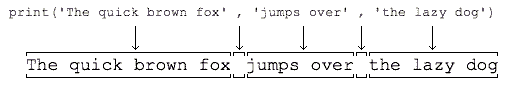
\includegraphics[width=0.6\linewidth]{fig/1017032122300544l.png}
\end{figure}


\texttt{print()}也可以打印整数,或者计算结果:

\begin{pythoncode}
>>> print(300)
300
>>> print(100 + 200)
300
\end{pythoncode}

因此,我们可以把计算\texttt{100\ +\ 200}的结果打印得更漂亮一点:

\begin{pythoncode}
>>> print('100 + 200 =', 100 + 200)
100 + 200 = 300
\end{pythoncode}

注意,对于\texttt{100\ +\ 200},Python
解释器自动计算出结果\texttt{300},但是,\texttt{\textquotesingle{}100\ +\ 200\ =\textquotesingle{}}是字符串而非数学公式,Python
把它视为字符串,请自行解释上述打印结果。

\hypertarget{ux8f93ux5165}{%
\subsubsection{输入}\label{ux8f93ux5165}}

现在,你已经可以用\texttt{print()}输出你想要的结果了。但是,如果要让用户从电脑输入一些字符怎么办?Python
提供了一个\texttt{input()},可以让用户输入字符串,并存放到一个变量里。比如输入用户的名字:

\begin{pythoncode}
>>> name = input()
Michael
\end{pythoncode}

当你输入\texttt{name\ =\ input()}并按下回车后,Python
交互式命令行就在等待你的输入了。这时,你可以输入任意字符,然后按回车后完成输入。

输入完成后,不会有任何提示,Python
交互式命令行又回到\texttt{\textgreater{}\textgreater{}\textgreater{}}状态了。那我们刚才输入的内容到哪去了?答案是存放到\texttt{name}变量里了。可以直接输入\texttt{name}查看变量内容:

\begin{pythoncode}
>>> name
'Michael'
\end{pythoncode}

** 什么是变量?** 请回忆初中数学所学的代数基础知识:

设正方形的边长为\texttt{a},则正方形的面积为\texttt{a\ x\ a}。把边长\texttt{a}看做一个变量,我们就可以根据\texttt{a}的值计算正方形的面积,比如:

若 a=2,则面积为 a x a = 2 x 2 = 4;

若 a=3.5,则面积为 a x a = 3.5 x 3.5 = 12.25。

在计算机程序中,变量不仅可以为整数或浮点数,还可以是字符串,因此,\texttt{name}作为一个变量就是一个字符串。

要打印出\texttt{name}变量的内容,除了直接写\texttt{name}然后按回车外,还可以用\texttt{print()}函数:

\begin{pythoncode}
>>> print(name)
Michael
\end{pythoncode}

有了输入和输出,我们就可以把上次打印\texttt{\textquotesingle{}hello,\ world\textquotesingle{}}的程序改成有点意义的程序了:

\begin{pythoncode}
name = input()
print('hello,', name)
\end{pythoncode}

运行上面的程序,第一行代码会让用户输入任意字符作为自己的名字,然后存入\texttt{name}变量中;第二行代码会根据用户的名字向用户说\texttt{hello},比如输入\texttt{Michael}:

\begin{pythoncode}
C:\Workspace> python hello.py
Michael
hello, Michael
\end{pythoncode}

但是程序运行的时候,没有任何提示信息告诉用户:``嘿,赶紧输入你的名字'',这样显得很不友好。幸好,\texttt{input()}可以让你显示一个字符串来提示用户,于是我们把代码改成:

\begin{pythoncode}
name = input('please enter your name: ')
print('hello,', name)
\end{pythoncode}

再次运行这个程序,你会发现,程序一运行,会首先打印出\texttt{please\ enter\ your\ name:},这样,用户就可以根据提示,输入名字后,得到\texttt{hello,\ xxx}的输出:

\begin{pythoncode}
C:\Workspace> python hello.py
please enter your name: Michael
hello, Michael
\end{pythoncode}

每次运行该程序,根据用户输入的不同,输出结果也会不同。

在命令行下,输入和输出就是这么简单。

\hypertarget{ux5c0fux7ed3}{%
\subsubsection{小结}\label{ux5c0fux7ed3}}

任何计算机程序都是为了执行一个特定的任务,有了输入,用户才能告诉计算机程序所需的信息,有了输出,程序运行后才能告诉用户任务的结果。

输入是 Input,输出是 Output,因此,我们把输入输出统称为
Input/Output,或者简写为 IO。

\texttt{input()}和\texttt{print()}是在命令行下面最基本的输入和输出,但是,用户也可以通过其他更高级的图形界面完成输入和输出,比如,在网页上的一个文本框输入自己的名字,点击
``确定'' 后在网页上看到输出信息。

\hypertarget{ux7ec3ux4e60}{%
\subsubsection{练习}\label{ux7ec3ux4e60}}

请利用\texttt{print()}输出\texttt{1024\ *\ 768\ =\ xxx}:

\begin{pythoncode}
# -*- coding: utf-8 -*-
\end{pythoncode}

\hypertarget{ux53c2ux8003ux6e90ux7801}{%
\subsubsection{参考源码}\label{ux53c2ux8003ux6e90ux7801}}

\href{https://github.com/michaelliao/learn-python3/blob/master/samples/basic/do_input.py}{do\_input.py}

